\documentclass[10pt]{article}
\usepackage[margin=1in]{geometry} 
\usepackage{amsmath,amsthm,amssymb,amsfonts}
\usepackage{enumitem} 
\usepackage{graphicx}
\graphicspath{ {../P2/} {../P3/} {../P4/}}
\usepackage{listings}
\usepackage{color}
 
\definecolor{codegreen}{rgb}{0,0.6,0}
\definecolor{codegray}{rgb}{0.5,0.5,0.5}
\definecolor{codepurple}{rgb}{0.58,0,0.82}
\definecolor{backcolour}{rgb}{0.95,0.95,0.92}
 
\lstdefinestyle{mystyle}{
    backgroundcolor=\color{backcolour},   
    commentstyle=\color{codegreen},
    keywordstyle=\color{magenta},
    numberstyle=\tiny\color{codegray},
    stringstyle=\color{codepurple},
    basicstyle=\footnotesize,
    breakatwhitespace=false,         
    breaklines=true,                 
    captionpos=b,                    
    keepspaces=true,                 
    %numbers=left,                    
    numbersep=5pt,                  
    showspaces=false,                
    showstringspaces=false,
    showtabs=false,                  
    tabsize=2
}
 
\lstset{style=mystyle}
 
\newcommand{\N}{\mathbb{N}}
\newcommand{\Z}{\mathbb{Z}}
\newcommand{\C}{\mathcal{C}}
\newcommand{\D}{\mathcal{D}}
\newcommand{\R}{\mathbb{R}}
 
\begin{document}
 
\title{Numerical methods for linear regression}
\author{[redacted]}
\maketitle
 
In this paper we explore methods for regression of simple linear models. In section 1, we begin by discussing a popular method for the numerical optimization of differentiable cost functions: gradient descent. We compare two variants of its implementation, batch gradient descent (BGD) and stochastic gradient descent (SGD), and discuss their convergence characteristics. In section 2, we benchmark the performance of gradient descent on the least squares fitting of simple linear models on generated data and compare its performance against the analytic solution. Since the generated data is known The simplicity of the data allows us to study the effect of model selection as we consider both polynomial basis functions and cosine basis functions for the fitted model. Finally, in sections 3 and 4, we explore the effect of L2- and L1-norm regularization, respectively, in model optimization and discuss their implications on the bias-variance tradeoff of the fitted parameters.

\section{Gradient Descent}

\section{Linear Basis Function Regression}

Linear models are a popular choice of regression model due to their computational simplicity and interpretability. In a linear model, the model $f$ used to predict the observed data is expressed as a linear combination of terms:
$$ f(w,x) = \sum_i w_ig_i(x) $$
where $g$ are basis functions that transform the input data $x$, and $w$ are weights on each term. Note that while $g$ may involve a nonlinear transformation of $x$; the model is considered a linear model as long as it is linear in the parameters $w$. We can express $f$ in matrix form as
$$f(w,x) = \Phi w$$
where the ith column vector of $\Phi$ is $g_i(x)$. 

In the fitting of $n$ pairs of $(x,y)$ observational data, we first choose the functional form via selection of the basis functions $g_i$, and subsequently fit our model parameters $w_i$ by minimizing the sum of the square error (SSE) between the model prediction and the observed output: 
$$ argmin_w \theta(w) = argmin_w \sum_n (y_n - f(w,x_n))^2$$ % todo: define indexing variables
Alternative formulations of the problem exist where we simultaneously consider the space of potential models in the fitting process, however, that is outside the scope of this work.

The minimization of $\theta$ for linear basis functions has a closed form solution (Equation [below]). In the subsequent sections, we explore the tradeoffs between different choices of basis functions, and we use the analytically computed weights for various choices of linear basis function to benchmark gradient descent minimization of $\theta$ and gain intuition on its convergence properties. 

$$w = (\Phi^T\Phi)^{-1}\Phi^Ty$$

\subsection{Linear regression with a polynomial basis}

Eleven data points were generated under the following function with added noise:


$$f(x) = cos(\pi x) + cos(2\pi x); x \in [0,1]$$



Ignoring the true basis, we instead try to fit the data using a polynomial basis $\phi_0(x) = 1, \phi_1(x) = x, \phi_2(x) = x^2, ... , \phi_M(x) = x^M$, with GLS.  Figure 1 shows the tradeoff between model complexity and the quality of fit to the *training data*. At M=0 and M=1, the model is too simple and we have a large SSE. At the other extreme, with M=10, the model is able to exactly fit in the input data (SSE=0), however, with this little data, we are extremely susceptible to overfitting to the noise in the input data. Indeed, at high values of M, our fitted polynomials oscillate between points, thus deviating from the true model even within the range of the training data. Furthermore, since we know the true model is a sum of cosines, the extrapolative power of any of these polynomial basis models outside the training range of $x \in [0,1]$ is poor, thus underscoring the danger of using a model to predict outside the range of its training data.

\begin{figure}
\caption{As the polynomial order M increases, the sum of square error (SSE) between the fitted polynomial and the input data decreases, however the risk of overfitting increases.}
\begin{center}
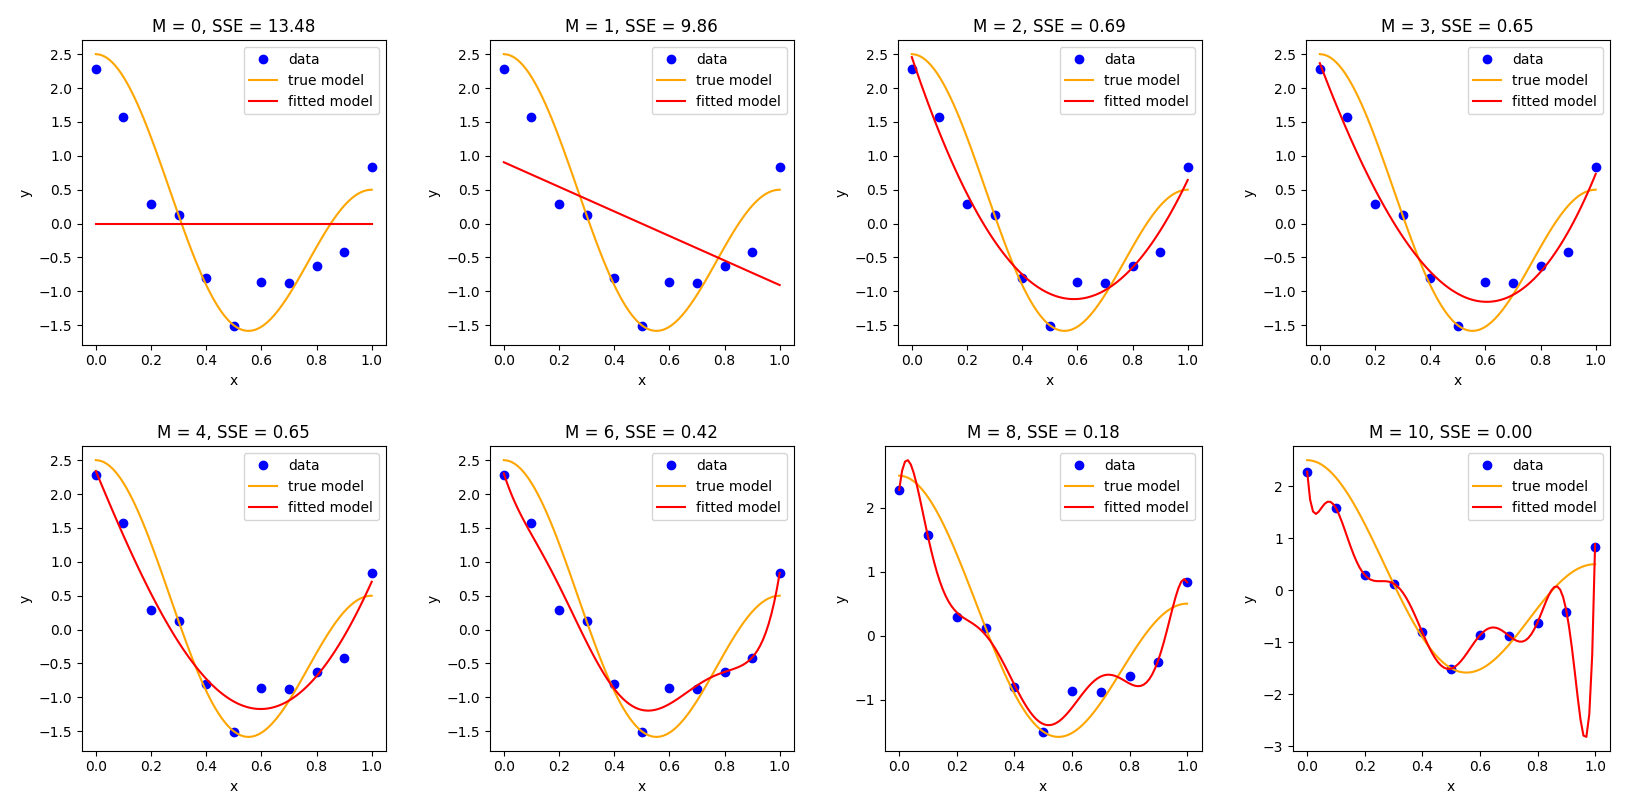
\includegraphics[width=450px]{all_regress_m}
\end{center}
\end{figure}

%\begin{table}
%\caption{Fitted weight vectors for linear regression of Equation [ref] with linear basis functions of increasing order.}
%\begin{center}
%\begin{tabular}{r | l}
%M=0 &  w =  [-0.001] \\
%M=1 &  w =  [0.906, -1.813] \\
%M=2 &  w =  [2.456, -12.15, 10.338] \\
%M=3 &  w =  [2.367, -10.731, 6.616, 2.481] \\
%M=4 &  w =  [2.341, -9.819, 2.055, 9.779, -3.649] \\
%M=6 &  w =  [2.304, -12.728, 63.938, -335.924, 783.22, -784.539, 284.565] \\
%M=8 &  w =  [2.278, 38.737, -972.518, 7401.42, -27960.868, 58014.38, -67074.038, 40504.018, -9952.576] \\
%M=10 &  w =  [2.278, -73.082, 2283.818, -30586.685, 208190.139, -813749.26, 1934260.6, -2841219.608, 2518054.828, -1233682.014, 256519.873] \\
%\end{tabular}
%\end{center}
%\label{poly_weights}
%\end{table}


\subsection{Performance of BGD and SGD}

Next we explore the performance of BGD and SGD on the same fitting problem with linear polynomial basis functions. The optimized values of $w$ are shown in Table {ref}. We note that both BGD and SGD have trouble reproducing the optimal values of $w$ for higher order polynomials. This is a consequence of both having a model that is too complex for the given data and the stopping criterion in gradient descent methods; since there are a large number of higher order polynomials that can approximate our 11 data points, the SSE between any two of these functions will be small. As a result, changing the starting values of affects the optimized values of $w$. Additionally, if the convergence threshold is set to an extremely low value, the number of iterations goes up drastically since the gradient between near optimal solutions is very low (Figure). SGD is less susceptible to this problem since the algorithm is inherently noiser. Finally, since our underlying data was generated from a cosine basis, i.e. even functions, we note that odd values of M required more/fewer iterations to convergence.

% table with BGD weights and SGD weights 
% Figure with number of iterations vs. tolerance for different values of M

\subsection{Linear regression with a cosine basis}

Using a cosine basis of the form $\phi_1(x) = cos(\pi x), \phi_2(x) = cos(2\pi x), ... , phi_M(x) = cos(M\pi x)$, we fit the same data as in Section 2.1 (Figure 2). Since the cosine basis contains the true basis used to generate the data, we observe low SSE for $M>=2$ and a good qualitative match to the true model for intermediate values of M. At larger values of M, we start overfitting to the noise in the generated data. For example, at M=8, $w_{opt} =  (0.769, 1.087, 0.099, 0.143, -0.051, 0.362, 0.012, 0.015) $. While $w_1=0.77$ and $w_2=1.09$ are close to the true model $w_1 = w_2 = 1$, higher order terms have nonzero weight. In the next section, we discuss how regularization techniques may be used to enforce prior beliefs on our model parameters to avoid overfitting to noise.

\begin{figure}
\caption{As the cosine order M increases, the sum of square error (SSE) between the fitted model and the input data decreases, however the risk of overfitting increases.}
\begin{center}
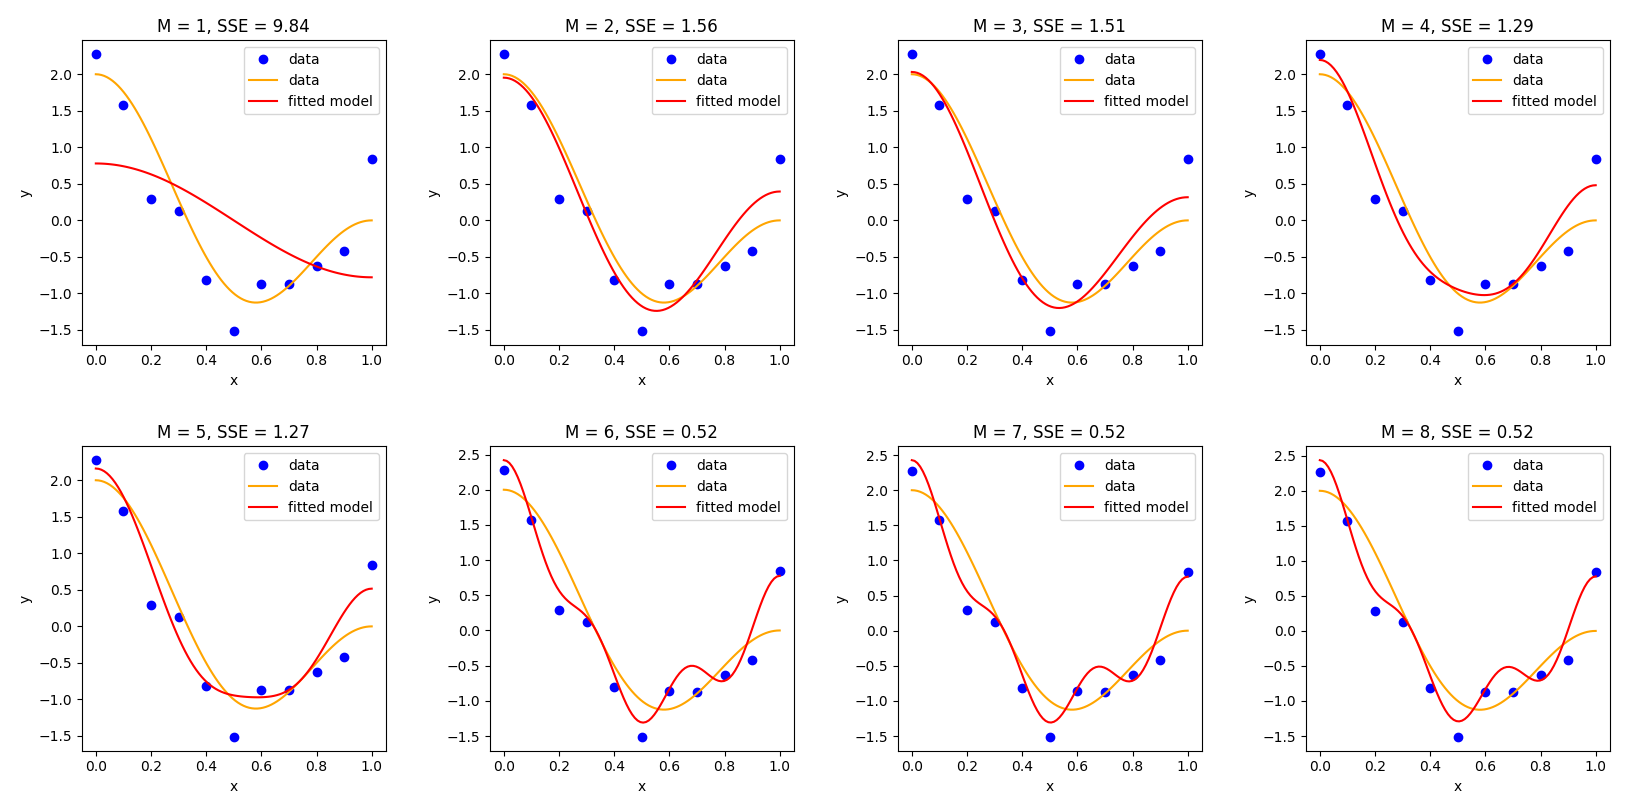
\includegraphics[width=450px]{all_regress_cos}
\end{center}
\end{figure}

%\begin{table}
%\caption{Fitted weight vectors for linear regression of Equation [ref] with cosine basis functions of increasing order.}
%\begin{center}
%\begin{tabular}{r | l}
%
%M=1 &  w =  [0.779] \\
%M=2 &  w =  [0.779, 1.174] \\
%M=3 &  w =  [0.763, 1.174, 0.094] \\
%M=4 &  w =  [0.763, 1.141, 0.094, 0.197] \\
%M=5 &  w =  [0.77, 1.141, 0.101, 0.197, -0.049] \\
%M=6 &  w =  [0.77, 1.089, 0.101, 0.145, -0.049, 0.363] \\
%M=7 &  w =  [0.769, 1.089, 0.099, 0.145, -0.051, 0.363, 0.012] \\
%M=8 &  w =  [0.769, 1.087, 0.099, 0.143, -0.051, 0.362, 0.012, 0.015] \\
%\end{tabular}
%\end{center}
%\label{cosine_weights}
%\end{table}

\section{Ridge Regression}

Ridge regression is a simple extension of generalized least squares which includes a second order regularization term to the error function. The relative importance of this regularization term is controlled by a parameter $\lambda$. 

$$f(w,x) = \Phi w + \lambda w^Tw$$

In a Baeysian framework, ridge regression represents including a prior that our weight parameters come from a gaussian distribution. In a frequentist framework, ridge regression is interpreted as adding a bias to our weight parameters in order to reduce the variance in our optimized weights. An advantage of regularization is that it allows model complexity to be tuned by adjusting the value of $\lambda$. In this section, we see how adding regularization affects our regressed parameters and how it allows us to fit a complex model to our data without severe overfitting.

We performed ridge regression with a polynomial basis on the same data set as in Section 2.1. We see that at M=8, using ridge regression dramatically reduces the magnitude of the fitted parameters and avoids overfitting. At sufficiently high values of lambda, we see our error function increase and the quality of fit decrease as our fitted function approaches a flat line.

% Figure: data fitted at M = 8 with different values of lambda
% Figure: total error, bias, variance vs lambda for different values of M

Next, we explore the optimization of our model parameters, $M$ and $\lambda$, by a data set split into a training (A), validation, and test (B) set. We measured the performance of each training on A and testing on B and vice versa, with validation performed on the validation set.


% training table for different values of M and lambda on training set: AIC, BIC, error
% validation table for different values of M and lambda on training set: AIC, BIC, error

% Figure: training error, testing error vs lambda... TODO

%We ran our ridge regression with a polynomial basis function on three datasets A, B and validation and tested the performance, as measured by $R^2$, in the following cases: training and regressing on A, training on A and regressing on B, training on A and regressing on validation, training and regressing on B, training on B and regressing on A, training on B and regressing on validation (Figure \ref{fig:3.2}). This was repeated for all parameter combinations of $M \in \{3,5,50\}$ and $\lambda \in \{0.1,10,100\}$. From the bottom two rows of the table, the highly negative $R^2$ values for $m=50$ make it clear than ridge regression heavily punishes model that severely overfit the data. Much better performance is seen with much more reasonable $M$ values such as 3 and 5. 

%\medskip

%However, it is also clear that there is danger in choosing a $\lambda$ value that is too high. From the top four rows of the table we can see that when $\lambda=10$ the model with $M=5$ outperforms the model with $M=3$ on the validation data. On the other hand, when $\lambda=100$ the model with $M=3$ is better than the one with $M=5$. However, this model is still performs worse on the validation set than both of the models generated with $\lambda = 10$. This illustrates that while increasing $\lambda$ is good for preventing overfitting, doing so runs the risk of generating a model with little predictive power.


\section{Sparsity and LASSO}

While the regularization in ridge regression penalizes high value parameters, LASSO regularization promotes sparsity by driving coefficients of certain basis functions to zero.

We trained, validated, and tested a dataset generated according to $y=w_{true}^T\phi(x) + \epsilon$, where $x,y \in \R, w \in \R^{13}$ and $\epsilon$ is a small noise. The feature vector is given by
$$ \phi(x) = (x, sin(0.4\pi x), sin(2*0.4\pi x), sin(3*0.4\pi x),...,sin(12*0.4\pi x)) \in \R^13$$

\begin{figure}
\caption{Training LASSO and ridge regularization.}
\begin{center}
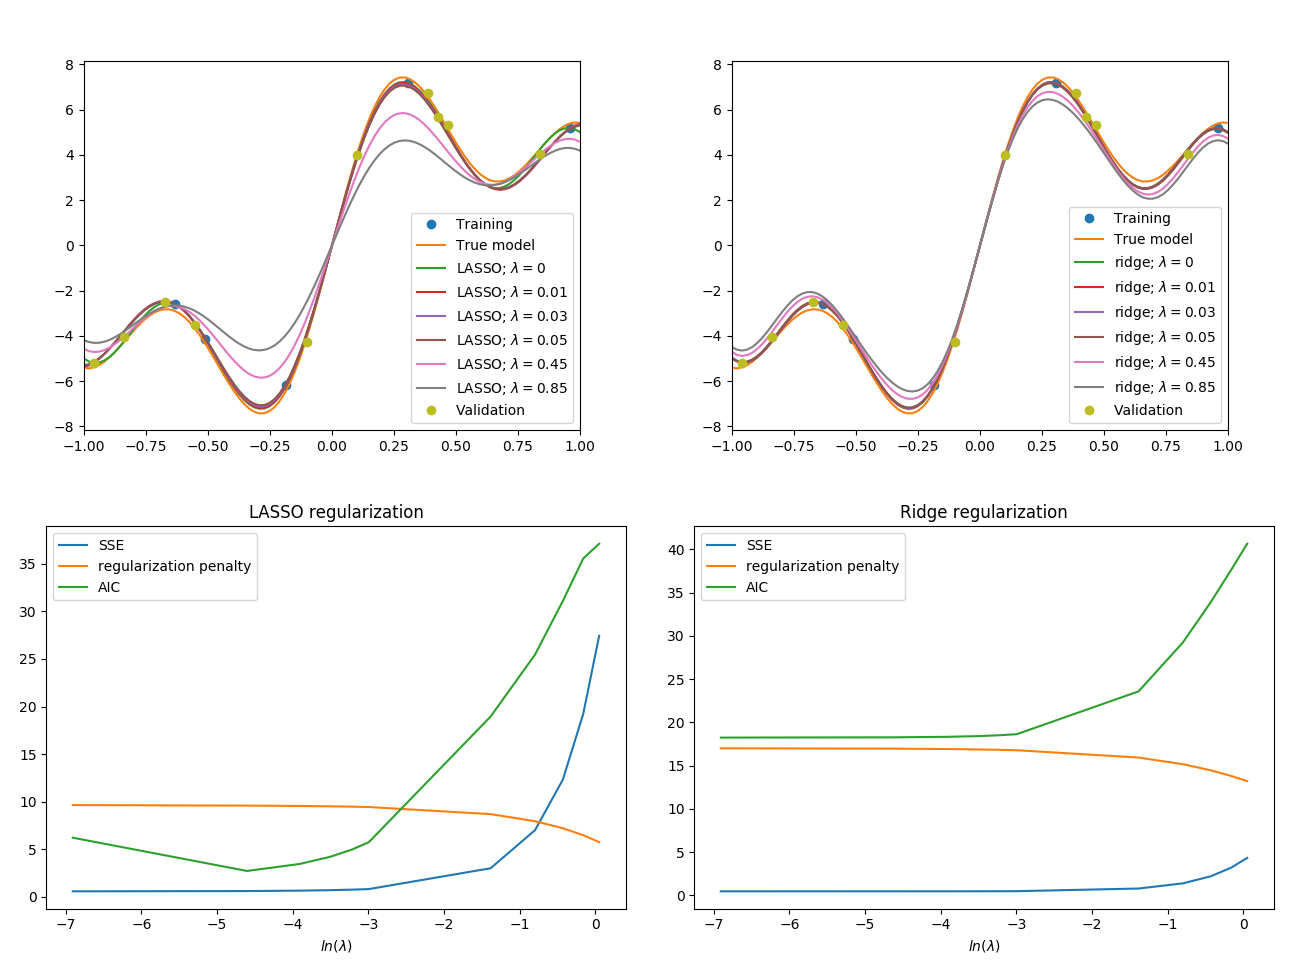
\includegraphics[width=350px]{all_training}
\end{center}
\label{fig:train_lasso}
\end{figure}

Our training results for various values of $\lambda$ for LASSO and ridge regularization are given in Figure \ref{fig:train_lasso}. After training each model, we use the validation data set to evaluate each set of parameters and choose an appropriate model. We see an inverse relationship between goodness of fit to the data and the regularization penalty. In order to compare different models, we compute the Akaike information criterion (AIC) to assess the tradeoff between goodness of fit and model complexity. Based on our computed AIC, we select the model with $\lambda=0.01$ for LASSO and $\lambda=0.01$ for ridge regression.

\begin{figure}
\caption{Fitting results.}
\begin{center}
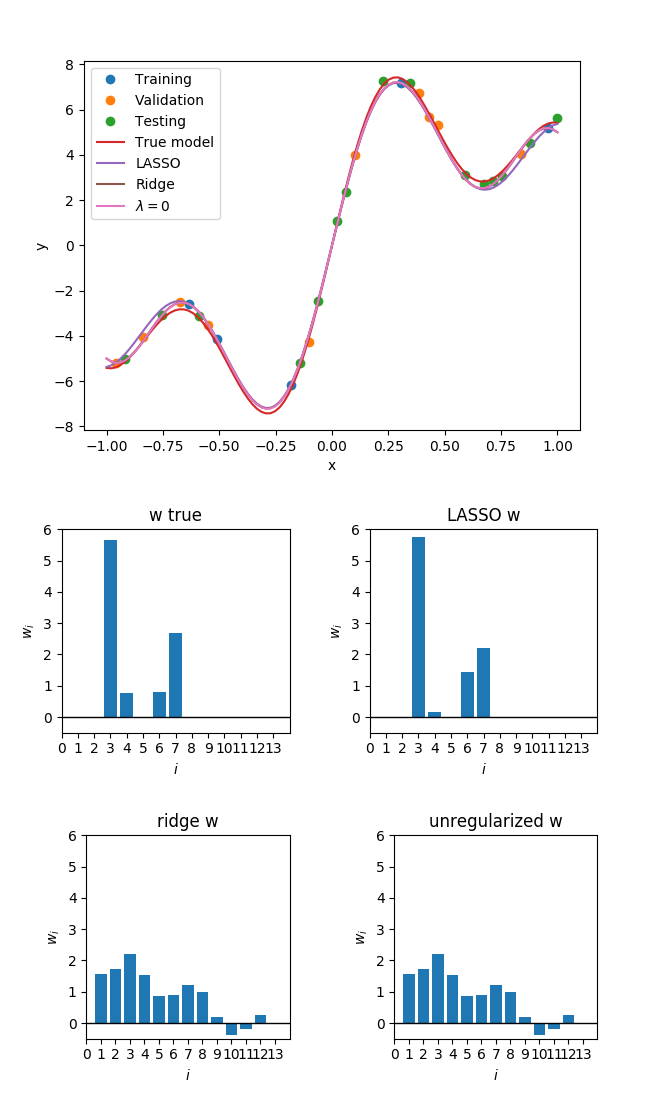
\includegraphics[width=200px]{final_fitting_results}
\end{center}
\label{fig:final_lasso_test}
\end{figure}

The optimized weights for each model is given in Figure \ref{fig:final_lasso_test} and a visualization of the fitted functions. While all models achieve a low error to the given data and qualitative agreement to the true model, visualizing the weights in the function shows that LASSO has most closely reproduced the true model. We also note that unregularized fitting yields parameters similar to ridge regression. This is likely a consequence of a small training set. We recommend combining the training and validation data sets used here and performing 3-fold cross validation for future work.

 %Finding the optimal LASSO weights has no closed form solution.

\section{Conclusions}

We have introduced batch gradient descent and stochastic gradient descent, two numerical methods used in the optimization of loss functions. We then introduced how gradient descent can be used in the context of generalized least squares and compared its performance for regression on linear models where there exists a closed form solution. We explore the relationship between the complexity of the model and the degree of overfitting in this data-poor context, thus motivating the introduction of regularization. We show how changing the regularization penalty tunes the model complexity, in particular, how ridge biases towards small parameter values and how ridge biases towards sparse values.

 \end{document}